% The two workflows of dSIBP: the full loop-momentum workflow (upper chain) and the
% time-only tree workflow (lower chain). The reduction backend runs outside the package.
\documentclass[tikz,border=8pt]{standalone}
\usetikzlibrary{arrows.meta,positioning,fit,backgrounds,calc}
\begin{document}
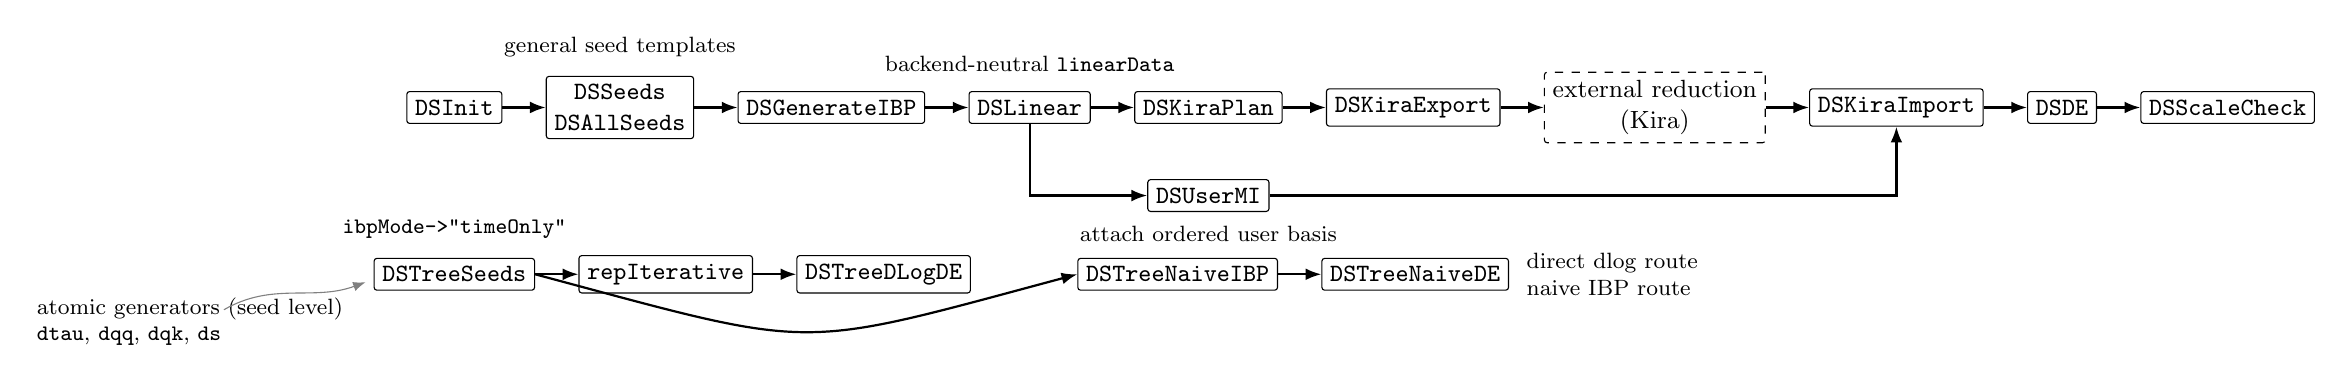
\begin{tikzpicture}[
  node distance=6mm and 5.5mm,
  box/.style={draw,rounded corners=1pt,align=center,inner sep=3pt,font=\small\ttfamily},
  ext/.style={draw,dashed,rounded corners=1pt,align=center,inner sep=3pt,font=\small},
  grp/.style={draw,gray,rounded corners=2pt,inner sep=4pt},
  arr/.style={-{Latex[length=2mm]},thick},
  note/.style={font=\footnotesize,align=center},
  yscale=1.0
]
% ---------- upper chain: full mode ----------
\node[box] (init) {DSInit};
\node[box,right=of init] (seeds) {DSSeeds\\DSAllSeeds};
\node[box,right=of seeds] (gen) {DSGenerateIBP};
\node[box,right=of gen] (lin) {DSLinear};
\node[box,right=of lin] (plan) {DSKiraPlan};
\node[box,right=of plan] (exp) {DSKiraExport};
\node[ext,right=of exp] (kira) {external reduction\\(Kira)};
\node[box,right=of kira] (imp) {DSKiraImport};
\node[box,right=of imp] (de) {DSDE};
\node[box,right=of de] (scale) {DSScaleCheck};
\draw[arr] (init) -- (seeds);
\draw[arr] (seeds) -- (gen);
\draw[arr] (gen) -- (lin);
\draw[arr] (lin) -- (plan);
\draw[arr] (plan) -- (exp);
\draw[arr] (exp) -- (kira);
\draw[arr] (kira) -- (imp);
\draw[arr] (imp) -- (de);
\draw[arr] (de) -- (scale);
\node[note,above=1.2mm of seeds] {general seed templates};
\node[note,above=1.2mm of lin] {backend-neutral \texttt{linearData}};
% user MI attachment
\node[box,below=7mm of plan] (usermi) {DSUserMI};
\draw[arr] (lin.south) |- ($(usermi.west)+(-3mm,0)$) -- (usermi.west);
\draw[arr] (usermi.east) -| ($(imp.south)+(0,-3mm)$) -- (imp.south);
\node[note,below=0.5mm of usermi] {attach ordered user basis};
% ---------- lower chain: time-only tree workflow ----------
\node[box,below=17mm of init] (tseeds) {DSTreeSeeds};
\node[box,right=of tseeds] (iter) {repIterative};
\node[box,right=of iter] (tdlog) {DSTreeDLogDE};
\node[box,right=of tdlog,xshift=8mm] (tnaive) {DSTreeNaiveIBP};
\node[box,right=of tnaive] (tnaivede) {DSTreeNaiveDE};
\draw[arr] (tseeds) -- (iter);
\draw[arr] (iter) -- (tdlog);
\draw[arr] (tseeds.east) to[out=-15,in=195,looseness=1.4] (tnaive.west);
\draw[arr] (tnaive) -- (tnaivede);
\node[note,right=1mm of tnaivede,align=left] {direct dlog route\\naive IBP route};
\node[note,above=1.2mm of tseeds] {\texttt{ibpMode->"timeOnly"}};
% ---------- atomic operators annotation ----------
\node[note,align=left,anchor=west] at ($(tseeds.west)+(-44mm,-6mm)$)
  {atomic generators (seed level)\\
   \texttt{dtau}, \texttt{dqq}, \texttt{dqk}, \texttt{ds}};
\draw[gray,thin,-{Latex[length=1.6mm]}] ($(tseeds.west)+(-19mm,-4.5mm)$) to[out=30,in=200] ($(tseeds.west)+(-1mm,-1mm)$);
\end{tikzpicture}
\end{document}
